\documentclass[11pt]{article}
\usepackage[margin=1.5in]{geometry}
\usepackage[utf8]{inputenc}
\usepackage{graphicx}
\usepackage{authblk}
\begin{document}

\title{ARM11 Project Final Report}
\author{C group 03}
\affil{Andy Chen, HouWang Wong, Jeshuran Jebanesan, Jiaju Yang}

\maketitle

\section{Abstract}
The aim of this project is to develop an ARM11 assembler that can decode basic ARM11 assembly language and translates into binary machine code. The task is done in a two-pass algorithm: recording any symbol for branch instructions and store them into a table in the first pass, and replacing these symbols with their corresponding value during the translation process in the second pass. The general translation logic as well as the usage of function pointers with respect to different kinds of instructions are very much similar to the first half of the project, albeit reversed. In addition, a three-player chess game for a hexagonal 96-tile board is implemented as a C program extension, which includes the board logic code that handles chess move logic, socket programming to enable communication between machines during multiplayer, and a chessboard GUI designed in Unity engine.
\section{Assembler}
\subsection{General structure}
For the assembler, a test-driven approach was taken, where the testing framework for the functions were designed first, then the functions themselves were defined. From the development experience in the first half of the project and the test suite used in many of the PPTs, the fact that only a few function tests were performed before debugging stage would result in a long debugging time due to the difficulty of pinning down the problematic parts of the code.\newline
As shown in figure 1, the structure was divided into 4 main parts: 
    
\begin{figure}
\centering
\begin{minipage}{.5\textwidth}
\centering
\includegraphics[width = \linewidth]{ Assembler_structure }
\caption{Assembler workflow chart}
\end{minipage}\hfill
\end{figure}

\subsubsection{First pass: Parser and Tokenizer}
In the first pass, the assembly file was read line by line until the end of the file. The number of words in each line was kept track of. If there was only one word in a line, that line would be a label. If so, the label would be added to the symbol table. If the line was a normal instruction instead, then the opcode and operands would be stored inside a singly linked list representing the disassembled lines.
\subsubsection{Second pass}
In the second pass, the linked list of disassembled lines were processed in a recursive manner. Each line was mapped to the corresponding translate function pointer and a default condition binary code. The function is then executed to produce the required binary. This made the functions more independent and making it easier to carry out function testings.
    
\subsubsection{Translate functions}
Similar to the emulator, the assembly lines and the respective functions are categorized into 4 main types: data process, data transfer, multiply and branch, and function pointers were applied as well. A triple map was also present for the program to search for the appropriate pointer with respect to the opcodes. There were several similarities in how different categories of lines are decoded so helper functions were created to reduce code duplication.

\subsubsection{Output}
The binary lines would then be converted to little-endian format and printed out into the output file.
    
\begin{figure}
\centering
\begin{minipage}{.5\textwidth}
\centering
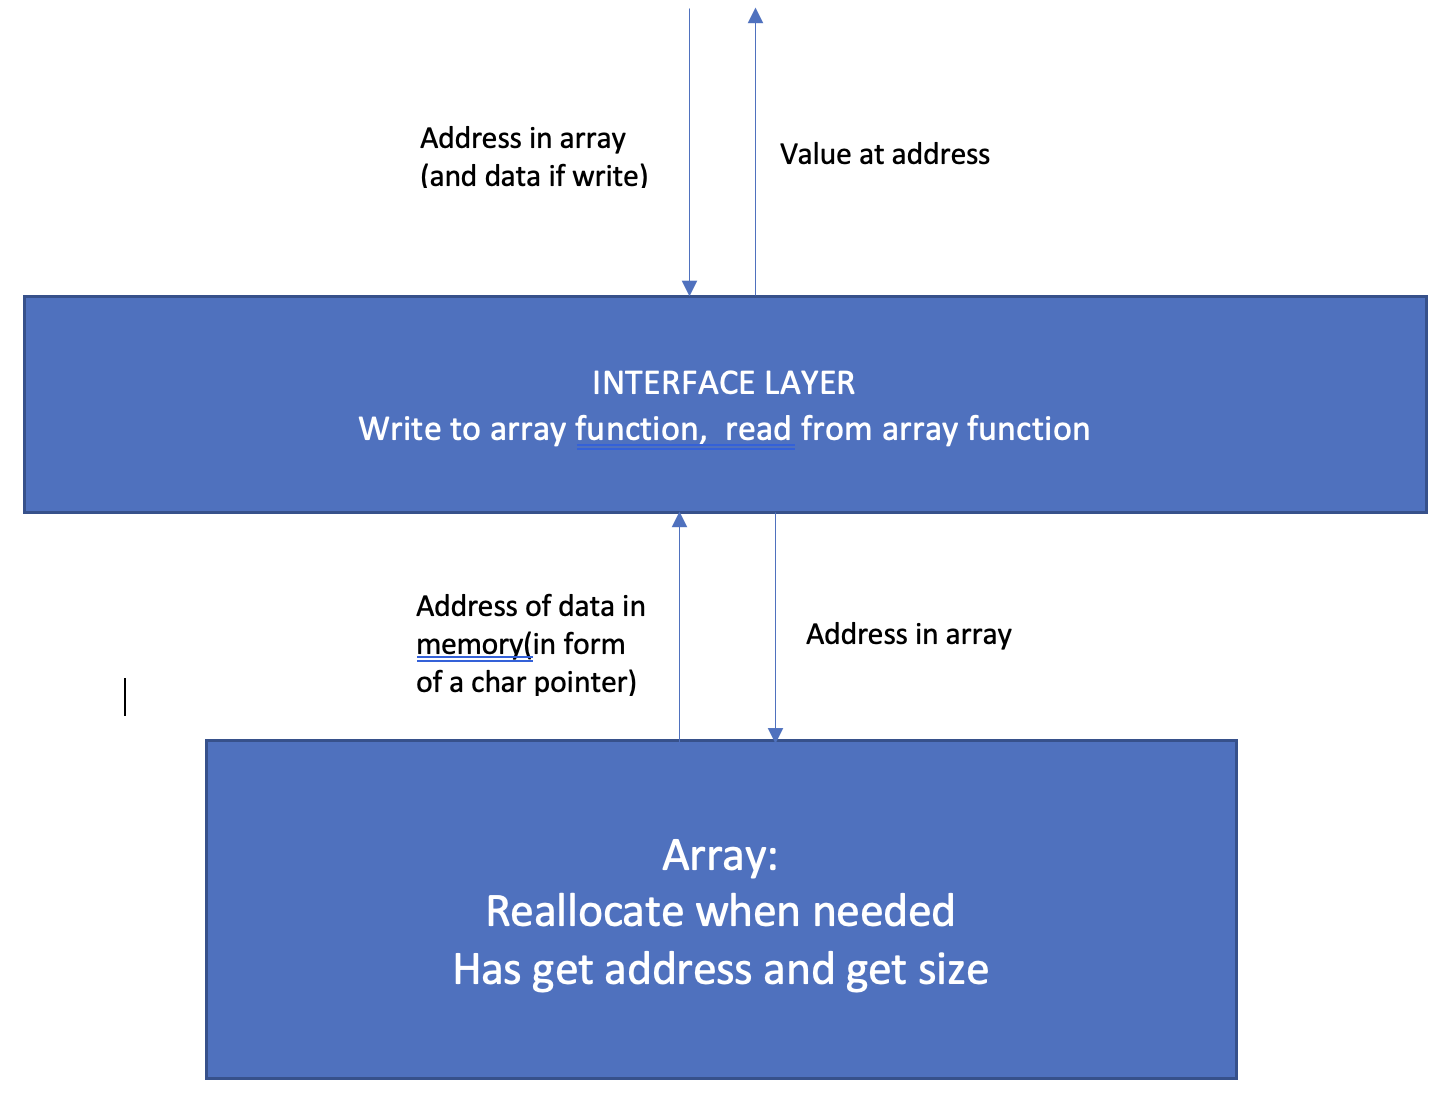
\includegraphics[width = \linewidth]{ mem_array }
\caption{Encapsulated structure of the polymorphic memory array}
\end{minipage}\hfill
\end{figure}

\subsection{Challenges}
A problem was to choose the appropriate form of data representation for assembly lines. The original method was to use a dynamic array like the memory array that was implemented early on. This required the assemble lines to be looped through twice which reduced efficiency. We got around this by using the linked list. Even though a linked list complexity is higher than static array, the assemble lines are read sequentially, which makes the execution time similar to a static array.\newline
For the symbol table, we used the memory array data structure from the emulator because:
    
1. The size of array is unknown, which could be solved with memory array's internal reallocation function.
    
2. Memory array can be used to store any type of element. The type conversion would be defined at the interface shown in figure 2.
\pagebreak

\section{Extension: Three-player Chess}
\subsection{General structure}
The theme chosen for the extension part of the project is a three-player chess game played on a hexagonal, 96-tile chessboard featuring online multiplayer.

\end{document}